\section{Hardware-Software Mapping}
\label{sec:HardwareSoftwareMapping}

For better understanding, in this section the abstract components as shown in Figure \ref{fig:subsystemDecomposition} are mapped to concrete components in an exemplatory execution environment. Therefor, the target client environment is defined as the Apple ecosystem, particularly the development of iOS, iPadOS or macOS-based client applications.  A common use case for this environment is the integration of resource-based Web APIs in the REST architectural style that are described by the OpenAPI \ac{IDL}. Swift is used as the target programming language in which to output the result and to import previous versions of the facade code. By restricting to these criteria, the subsystem decomposition now contains more specific components as shown in Figure \ref{fig:subsystemConcrete}. 

\begin{figure}[!h]
	\centering{
		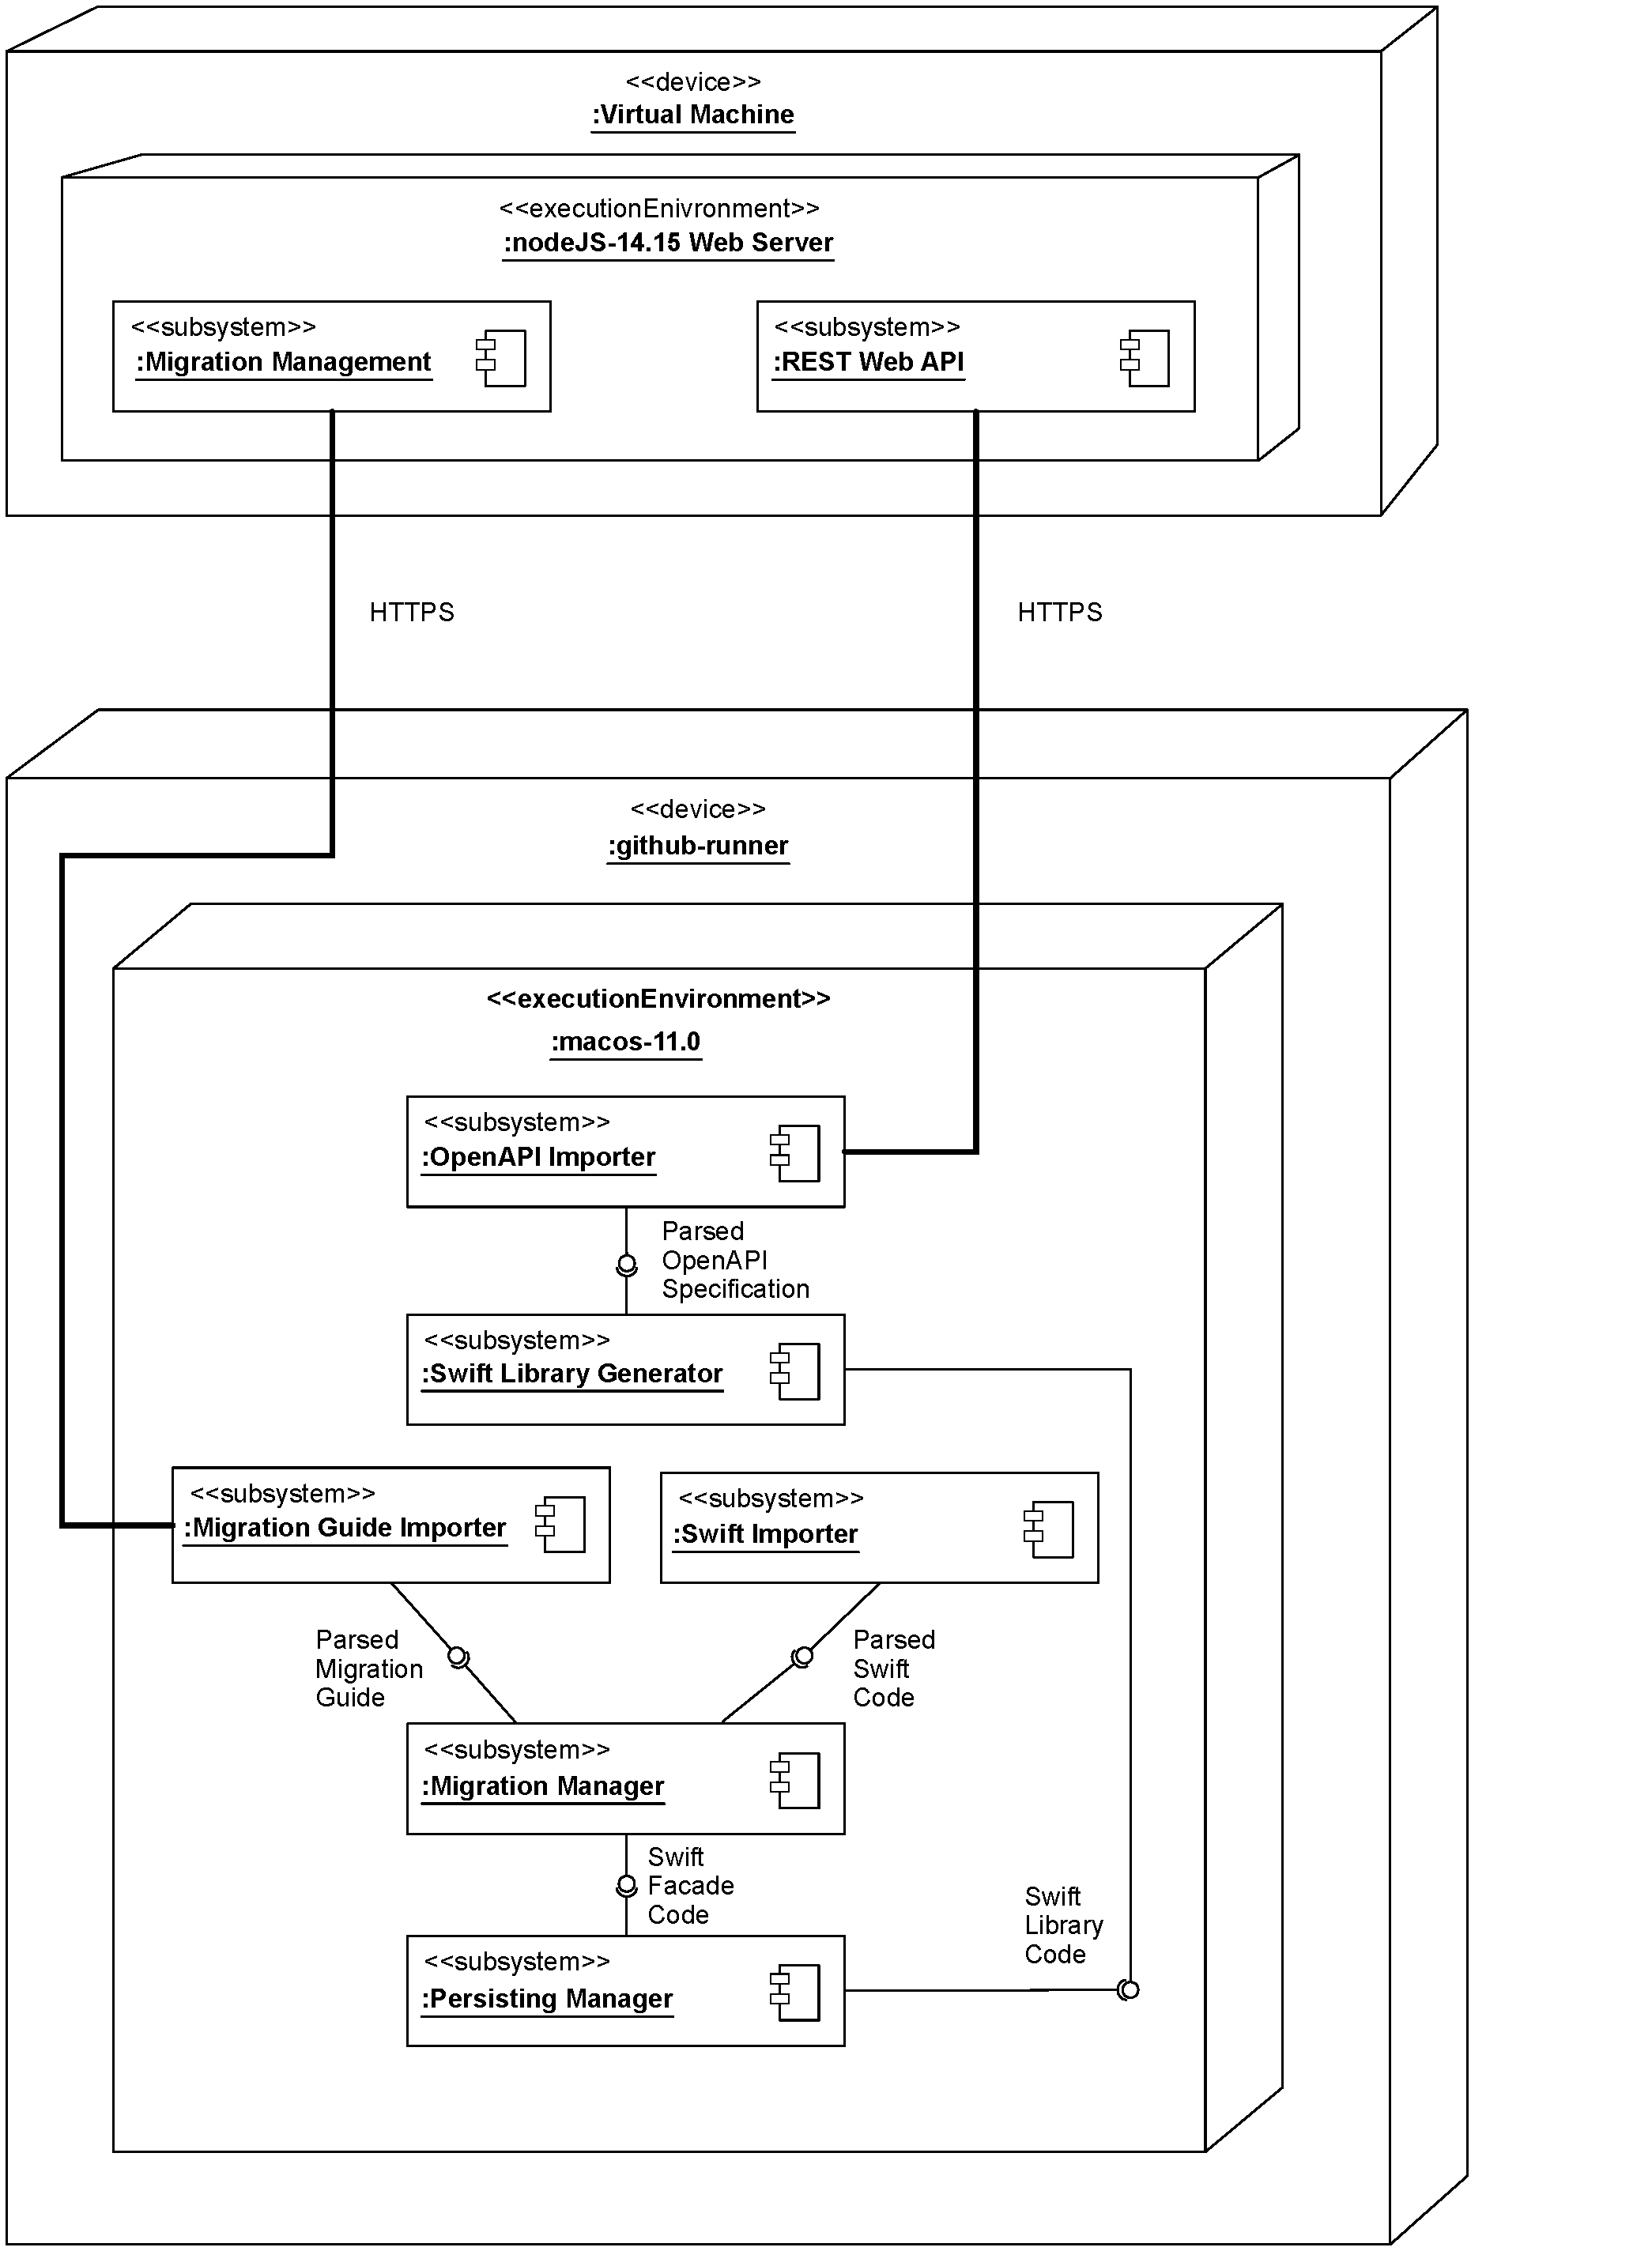
\includegraphics[width=150mm]{images/subsystem_concrete.pdf}
		\caption{Subsystem decomposition in an Apple ecosystem}
		\label{fig:subsystemConcrete}
	}
\end{figure}

The Web API is built using the \ac{REST} architectural style. It is served by a \texttt{nodeJS} web server hosted on a virtual machine maintained by the Web API provider. Its functionality is described using the OpenAPI \ac{IDL}. This document is published on a separate URI of the Web API. Additionally, a \texttt{Migration Management} subsystem is used to track all changes that have been introduced to the Web API. It notes all changes in a machine-readable migration guide and publishes it on a separate URI. Both document can be retrieved using \texttt{HTTPS}. 

In order to import the specification document, the OpenAPI Importer subsystem must be able to parse specifications using both, the \textit{\ac{JSON}} and \textit{\ac{YAML}} documentation styles. While the system itself can be impemented using an arbitrary programming language, every subsystem that is concerned with importing or generating source code must support Swift. The \texttt{Swift} \texttt{Library} \texttt{Gen\-er\-ation} subsystem uses the parsed specification to create Swift files containing model and endpoint definitions that enable the interaction with the Web API. Appropriate tooling to generate a library from an OpenAPI specification is available for all major programming languages. The OpenAPI Generator\footnote{https://openapi-generator.tech/}, implemented using Java, is one of them, supporting 65 programming languages and dialects. It combines the functionality of the \texttt{OpenAPI} \texttt{Importer} and \texttt{Swift} \texttt{Library} \texttt{Gen\-er\-ation} subsystems.

Parsing a migration guide requires a custom implementation of the \texttt{Migration} \texttt{Guide} \texttt{Importer} as no reusable components exist yet. The subsystem responsible for importing the previous facade must support parsing Swift code. The internal behavior of it is modified according to the changes as stated in the encoded migration guide. After that, the adapted facade is transformed into the textual representation of Swift-based source code by the \texttt{Swift} \texttt{Facade} \texttt{Generator}. There are multiple tools available that support generating Swift code using Stencil templates. The most popular ones are SwiftGen\footnote{https://github.com/SwiftGen/SwiftGen} and Sourcery\footnote{https://github.com/krzysztofzablocki/Sourcery}. They provide similar features that enable users to generate Swift code based on several template types by executing the compiled application via CLI. Sourcery additionally offers a well-maintained framework to enable an integration into existing Swift applications.

The \texttt{Persisting} \texttt{Manager} subsystem uses a linting ruleset to format the library and facade code according to its configuration, before adding meta-files and creating a Swift package which can be imported by client applications using the \textit{\ac{SPM}}. Formatting code based on a linting ruleset is one feature of SwiftLint\footnote{https://github.com/realm/SwiftLint}, the most popular linter for Swift code. While it can be installed and used via CLI, it also supports an integration as a Swift package that enables developers to lint and format Swift code stored in its textual representation.